\section{Relate Other Data Structures with Extended Priority Queue}
\label{sec:relate other data structures with extended priority queue}

In this section, we shows how to reduce queue and stack executions into priority queue executions in polynomial time.


\subsection{Relate Queue with Extended Priority Queue}
\label{subsec:relate queue with extended priority queue}

Given a queue execution $e_q$, we can obtain an execution $\textit{QtoEPQ}(e_q)$ of extended priority queue by (1) transforming $\textit{enq}(a)$ and $\textit{deq}(a)$ into $\textit{put}(a,p)$ and $\textit{rm}(a)$ for each $a \in \mathbb{D}$, and (2) transforming $\textit{deq}(\textit{empty})$ into $\textit{rm}(\textit{empty})$. Note that in $\textit{QtoEPQ}(e_q)$, we assign all items with a same priority $p \in \mathbb{P}$. Since we have already guarantee that each single-priority execution of priority queue has FIFO property, it is easy to see that $e_q$ is linearizability w.r.t queue, if and only if $\textit{QtoEPQ}(e_q)$ is linearizable w.r.t $\textit{EPQ}$, as stated by the following lemma:

\begin{restatable}{lemma}{RelateQueuewithEPQ}
\label{lemma:relate queue with extended priority queue}
Given an execution $e_q$ of queue, $e_q$ is linearizable w.r.t queue, if and only if $\textit{QtoEPQ}(e_q) \sqsubseteq \textit{EPQ}$.
\end{restatable}


\subsection{Relate Multi-Set with Extended Priority Queue}
\label{subsec:relate multiSet with extended priority queue}

A multi-set contains two method: $\textit{insert}$ and $\textit{delete}$. A $\textit{insert}$ method has one argument, and is used to insert an item into the multi-set. We also assume that the item is chosen from a specific (possibly infinite) data domain $\mathbb{D}$. A $\textit{delete}$ method intends to remove an arbitrary item in multi-set and then returns it. If the multi-set is empty, $\textit{delete}$ returns $\textit{empty}$. Note that when $\textit{delete}$ returns an item, there is no restriction (such as FIFO, LIFO or priorities) for how to choose this item in multi-set.

Let $\textit{MSet}$ be the set of sequential executions of multi-set. In Appendix \ref{subsec:appendix proof and definition in section relate multiset with extended priority queue}, we give inductive rules of $\textit{MSet}$, and prove that these rules are step-by-step linearizability and co-regular. We also give witness automata for $\textit{MSet}$. Here we use the notion of inductive rules, step-by-step linearizability and co-regular in \cite{Bouajjani:2015}.

Since multi-set does not add any constraint for selecting item when deleting items, we simulate such behavior by giving each item an unique priority where such priorities are pair-wise incomparable. To make it simple, we just ignore items that are putted more than one times. Such ignorance is correct due to data-independence. Formally, given a multi-set execution $e_m$, we can obtain an execution $\textit{MStoEPQ}(e_m)$ of extended priority queue by (1) erasing operations of items which are putted more than once in $e_m$, (2) transforming $\textit{insert}(a)$ and $\textit{delete}(a)$ into $\textit{put}(a,p_a)$ and $\textit{rm}(a)$ for each $a \in \mathbb{D}$, and (3) transforming $\textit{delete}(\textit{empty})$ into $\textit{rm}(\textit{empty})$. Here we need to ensure that for each $a \neq b$, $p_a$ and $p_b$ must be incomparable. Given a set $S$ of executions of multi-set, let $\textit{MStoEPQ}(S)$ be the set generated by applying $\textit{MStoEPQ}$ to each sequence in $S$. Let $\textit{Auts}_{\textit{EPQ}}$ and $\textit{Auts}_{\textit{MS}}$ be the set of witness automata for extended priority queue and for multi-set, respectively. The following lemma stats that our witness automata for extended priority queue are enough for checking violations w.r.t $\textit{MSet}$.

\begin{restatable}{lemma}{RelateMultiSetwithEPQ}
\label{lemma:relate multi set with extended priority queue}
Given an data-independent implementation $\mathcal{I}_m$ of multi-set, $\mathcal{I}_m \cap \textit{Auts}_{\textit{MS}} \neq \emptyset$, if and only if $\textit{MStoEPQ}(\mathcal{I}_m) \cap \textit{Auts}_{\textit{EPQ}} \neq \emptyset$.
\end{restatable}


\subsection{Relate Stack with Extended Priority Queue}
\label{subsec:relate stack with extended priority queue}

A stack contains two method: $\textit{push}$ and $\textit{pop}$. A $\textit{push}$ method has one argument, and is used to insert an item into the stack. A $\textit{pop}$ method intends to remove an item that is newest in stack and then returns it. If the stack is empty, $\textit{pop}$ returns $\textit{empty}$.

Given an execution $e_s$ of stack, we can obtain an execution $\textit{StoEPQ}(e_s)$ of extended priority queue by transforming $\textit{push}(a)$ and $\textit{pop}(a)$ into $\textit{put}(a,p_a)$ and $\textit{rm}(a)$, and transforming $\textit{pop}(\textit{empty})$ into $\textit{rm}(\textit{empty})$. Here let us show the process of assigning priorities for items. Given $e_s$, the process of assign priorities is as follows: 

\begin{itemize}
\setlength{\itemsep}{0.5pt}
\item[-] Let $e'$ be the projection of $e_s$ into $\textit{push}$. For each $i$, associate the $\textit{i-th}$ element of $e'$ with $e$. 

\item[-] For each $\textit{push}_o(a)$ in $e$, we assign priority $(i,j)$ to it. Here $i$ and $j$ are the number associated with the call and return action of $\textit{push}_o(a)$. 
\end{itemize}  

Then the order $<_{\mathbb{P}}$ is defined as follows: $(i_1,i_2) <_{\mathbb{P}} (j_1,j_2)$, if $j_1 > i_2$, or we can say, if the $\textit{put}$ of the former happens before the $\textit{put}$ of the latter. In \figurename~\ref{fig:execution with intervals}, we associate numbers with the call and return actions of $\textit{put}$, and then assign priorities to items. We can see that the priority of $c$ is smaller than the priority of $a$ according to $<_{\mathbb{P}}$. 

\begin{figure}[htbp]
  \centering
  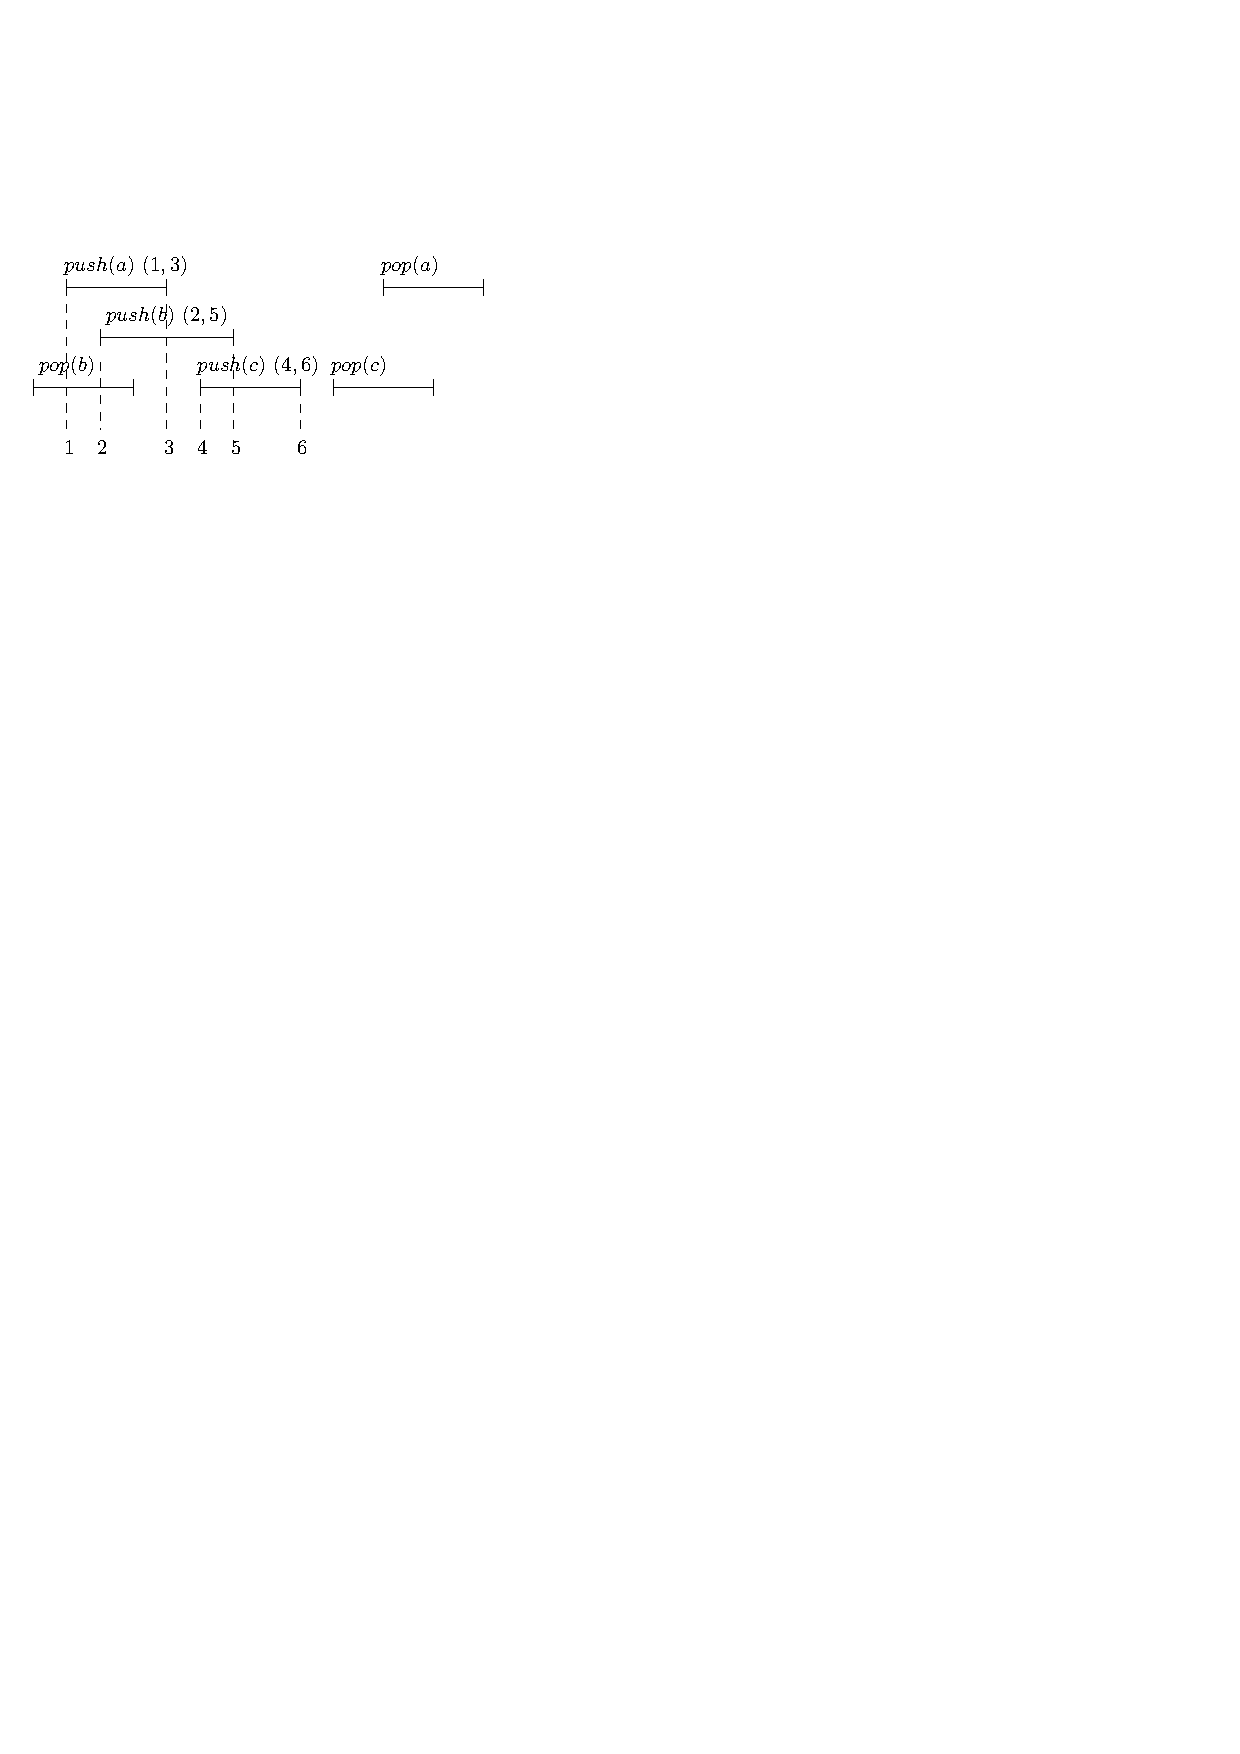
\includegraphics[width=0.6 \textwidth]{figures/PIC-HIS-INTRO-Interval.pdf}
%\vspace{-10pt}
  \caption{Execution with intervals}
  \label{fig:execution with intervals}
\end{figure}












